\documentclass[UTF8,11pt]{ctexart}

\usepackage[a4paper,margin=2.35cm]{geometry}
\usepackage{booktabs}
\usepackage{graphicx}
\usepackage{hyperref}
\usepackage{url}
\usepackage{array}
\usepackage{caption}
\usepackage{microtype}
\usepackage{xcolor}
\usepackage{longtable}
\IfFileExists{placeins.sty}{\usepackage{placeins}}{\newcommand{\FloatBarrier}{\clearpage}}
\newcommand{\PDAOfficialOverlap}{227}
\newcommand{\PDAWeekTwoAccuracy}{0.9830}
\newcommand{\PDAWeekTwoMacroFOne}{0.9743}
\newcommand{\PDAMobileParams}{2.27M}
\newcommand{\PDAMobileFlops}{0.31G}
\newcommand{\PDAMobileThroughput}{644.3}
\newcommand{\PDAFinalAccuracy}{0.9953}
\newcommand{\PDAFinalMacroFOne}{0.9941}
\newcommand{\PDAErrorCount}{50}
\newcommand{\PDATestCount}{10709}
\newcommand{\PDAECE}{0.0965}
\newcommand{\PDAMCE}{0.3348}
\newcommand{\PDABrier}{0.0140}
\newcommand{\PDADemoLatency}{129.8}
\newcommand{\PDAVLMChoice}{11/15}
\newcommand{\PDAVLMCondition}{1/5}
\newcommand{\PDAWeekEightCleanTests}{226}


\definecolor{evidenceblue}{HTML}{0066CC}
\hypersetup{colorlinks=true,linkcolor=evidenceblue,urlcolor=evidenceblue,citecolor=evidenceblue}
\setlength{\emergencystretch}{2em}
\renewcommand{\arraystretch}{1.15}

\title{PlantDiseaseAI：从高分分类器到可审计的植物病害研究系统}
\author{Panjoel}
\date{2026-07-19}

\begin{document}
\maketitle

\begin{abstract}
本文报告 PlantDiseaseAI 在 Week 1--8 的完整研究与工程证据。项目围绕 PlantVillage 受控背景图像建立数据审计、五模型统一基准、单变量消融、错误与校准分析、Grad-CAM 相关性可视化、MPS/Streamlit 演示、Apple container 复现以及 Qwen3-VL 小样本探索。后续 React/FastAPI 服务路径在冻结分类器外围增加目标叶片选择、植物身份路由、OpenCV 形态证据与拒识门控，但不改变既有 Benchmark。Week 2 ResNet50 在 official split 上获得 Accuracy \PDAWeekTwoAccuracy、Macro F1 \PDAWeekTwoMacroFOne；MobileNetV2 以 \PDAMobileParams 参数、\PDAMobileFlops FLOPs 和记录协议下 \PDAMobileThroughput~img/s 构成轻量候选。Week 3 的 Label Smoothing 与 Cosine Scheduler 组合在 seed 42、official split 上获得 Accuracy \PDAFinalAccuracy、Macro F1 \PDAFinalMacroFOne。然而数据审计发现 train/test 间有 \PDAOfficialOverlap 个重叠 leaf\_id，因此这些结果不是实体隔离泛化证据。Week 4 记录 \PDAErrorCount/\PDATestCount 个错误，并给出 ECE \PDAECE、MCE \PDAMCE、Brier \PDABrier。Week 5 的 \PDADemoLatency~ms 仅是一个固定合成输入的容器 CPU 观测。Week 6 Qwen3-VL choice/few-shot 冒烟严格匹配为 \PDAVLMChoice，condition 为 \PDAVLMCondition。Week 8 clean lane 共 \PDAWeekEightCleanTests 项测试通过，并完成本地证据与容器通道。本文的中心结论不是“高分即可信诊断”，而是：只有把数据边界、负结果、复现条件与安全拒答同时纳入，模型数字才具有可审计的研究意义。
\end{abstract}

\section{引言}

图像分类可为植物健康筛查提供低成本入口，但数据集高准确率并不自动等于可信的田间诊断。可信性至少包含四层含义：实验是否使用清晰且稳定的数据协议，指标是否能追溯到唯一运行记录，模型错误和置信度是否被审计，以及部署界面是否明确拒绝超出证据范围的建议。本项目据此把问题从“训练一个最高分模型”改写为“建立一个能说明自己何时有效、何时失效、如何复现的研究系统”。

PlantDiseaseAI 的分类主线按周推进。Week 1 固定数据加载、标签映射和评估接口；Week 2 在同一协议下比较五个 CNN；Week 3 以单变量消融支持模型选择；Week 4 审计错误、校准与 Grad-CAM；Week 5 将 Top-5、解释与安全提示整合进 Demo；Week 6 只在主线完成后探索视觉语言模型；Week 7 组织证据材料；Week 8 运行 clean、local evidence 与 Apple container 三条复现通道。本文将这些阶段组织为一条可核查的证据链，而非孤立的截图或最佳数字。

本文贡献有四点。第一，给出统一协议下的五模型基准和可解释的消融决策。第二，把数据重叠、逐样本错误、校准、解释目标层与固定输入延迟作为一等研究对象。第三，将代码测试、模型产物、图表、论文表述和本地容器验证连接到同一 release candidate。第四，明确区分已验证分类器证据、已实现服务门控与实验扩展，使目标叶片、身份、形态和建议阶段可以拒答，而不静默提高证据等级。所有结论都受 official split、单 seed 和受控背景限制；本文不声称真实田间泛化，也不提供农药名称、剂量或法规建议。

\section{相关工作}

PlantVillage 提供了开放的植物健康图像资源\cite{hughes2015plantvillage}。Mohanty 等人证明了深度卷积网络在该数据上的分类潜力，同时也指出训练分布与真实采集环境之间的差异\cite{mohanty2016plantdisease}。本项目采用 PlantVillage 的植物--病害闭集标签，但重点不是刷新数据集纪录，而是审计划分、比较模型、保存负结果，并把受控背景限制写入每个面向用户的入口。

架构比较覆盖 ResNet\cite{he2016resnet}、MobileNetV2\cite{sandler2018mobilenetv2} 和 EfficientNet\cite{tan2019efficientnet} 系列。训练策略包括 Label Smoothing\cite{szegedy2016label}、Focal Loss\cite{lin2017focal}、Cosine Scheduler\cite{loshchilov2017sgdr}、RandAugment\cite{cubuk2020randaugment}、Mixup\cite{zhang2018mixup} 与 CutMix\cite{yun2019cutmix}。这些方法在本文中被视为待验证因素，而不是默认有效的配方；同一预算下的下降结果与提升结果被共同保存。

可解释性使用 Grad-CAM\cite{selvaraju2017gradcam}，但热力图只表示目标分数与空间特征的相关性。置信度分析遵循现代神经网络校准研究\cite{guo2017calibration}，并明确区分 top-label calibration 与完整多类别概率校准。Week 6 使用 Qwen3-VL-4B-Instruct 模型卡所描述的视觉语言能力\cite{qwen3vl2025modelcard}，但实验规模只允许“本地冒烟探索”的措辞。

\section{数据集、任务与划分审计}

已验证任务是 38 类整图分类。输入是一张叶片图像，输出是 PlantVillage 闭集中的植物--病害类别概率。后续服务层会产生启发式目标叶片 mask、病斑候选与形态摘要，但它们不是学习得到的病理分割、病原检测或开放集保证。训练增强只作用于训练集，验证和测试使用确定性预处理；官方测试集不参与 checkpoint 选择或超参数搜索。

项目沿用数据源的 official train/test split，并在训练部分以 seed 42 做分层 train/validation 划分。审计通过样本标识追踪发现 official train/test 间有 \PDAOfficialOverlap 个重叠 leaf\_id。重叠并不等价于像素完全相同，但说明同一叶片实体的相关图像可能跨集合出现。因此本文统一使用“official split 结果”，而不使用“无泄漏”或“实体隔离”的表述。

这一风险直接影响研究解释。模型可能同时学习病斑视觉线索、拍摄背景和同实体相关特征；在受控背景上得到的数值不能推导到田间光照、遮挡、叶片姿态、相机差异或未知病害。后续正式研究的首要实验不是再堆叠更大模型，而是构建按 leaf entity 分组的冻结划分，并在多个随机种子和独立田间域上复验。

\subsection*{审计决策与更强划分协议}

本次审计保留来源标签与 official split，而不在看到测试结果后静默重写数据。此时更改划分会形成新协议，使既有运行失去直接可比性。下一版协议应先定义稳定实体键，把同一叶片的相关视图归入同一组，再按组而非按图片分配 train、validation 与 test；实体规则、数据版本、类别数、seed 与索引文件必须在模型选择之前冻结。

实体隔离也不是全部。新的 test 集仍须完全不参与模型与超参数选择；分组后要重新检查稀有类别支持度，避免 Macro F1 建立在过小样本上。重复审计应结合元数据与感知相似检查，不确定样本进入 ledger 而非自动删除。official-split 与 entity-isolated 结果应并列为两个协议，不能合并成一个标题数字。

\section{统一训练与评估协议}

训练、评估、推理和 Demo 共用标签映射、模型工厂、checkpoint 接口和确定性测试预处理。最佳 checkpoint 由 validation Macro F1 选择，随后仅在 official test split 上做最终评估。正式指标包括 Accuracy、Macro Precision、Macro Recall、Macro F1、分类别 Precision/Recall/F1、混淆矩阵与逐样本预测。Macro F1 为重要主指标，因为它降低大类别对总体结果的支配。

Week 3 的固定预算为 ResNet50、输入 224、batch size 16、5 epochs、AdamW、初始学习率 0.001 和 seed 42。单变量实验每次只改变一个因素；组合实验另行标识。随机性覆盖 Python、NumPy、PyTorch 与 DataLoader worker。MPS 测量使用 float32、batch-1 延迟、batch-32 吞吐、10 次预热和 50 次测量；由于 MPS 与 CUDA 的内存接口不同，本研究不报告未经可靠测量的峰值显存。

每个正式运行保存解析配置、split、标签映射、设备、软件环境、日志、指标和 checkpoint 索引。Week 8 又通过 manifest 对关键文件记录逻辑路径、大小与 SHA-256。这样，表格中的数字不能脱离其运行条件被复制成通用性能承诺。

\subsection*{协议不变量与失败记录}

共享实现避免训练、评估、推理和 Streamlit 各自维护预处理或标签顺序。checkpoint 加载校验模型元数据与类别数；Top-5 必须排序且概率有效；Grad-CAM hook 有明确生命周期，避免重复请求积累回调。这些工程不变量也是科研不变量：标签错位或归一化漂移可以在权重不变时产生看似合理但无效的结果。

运行状态区分 completed、failed、aborted 与 smoke-tested。失败运行不从历史中删除，smoke 也不提升为完整实验。MPS 可复现不代表跨设备逐位一致，容器健康检查不代表生产负载能力。把这些差异写进报告，可阻止后续材料静默提高证据等级。

\section{五模型基准}

\input{../tables/week2_benchmark_zh.tex}

ResNet50 在统一协议下获得最高测试表现：Accuracy \PDAWeekTwoAccuracy、Macro F1 \PDAWeekTwoMacroFOne，因此成为后续高精度消融基线。MobileNetV2 则以 \PDAMobileParams 参数、\PDAMobileFlops FLOPs 和记录的 \PDAMobileThroughput~img/s 吞吐形成部署候选。二者回答不同问题：前者服务于“当前预算下精度上限”，后者服务于“资源受限时的效率权衡”。

表中的延迟和吞吐只在记录的 MacBook MPS、输入尺寸、精度、预热与测量次数下可比。它们不能直接换算为手机、服务器或容器 CPU 性能。五个架构使用相同 split 和评估协议，因而可用于本项目内部模型选择，但 official split 的实体重叠限制仍同时作用于所有模型。

\subsection*{精度--效率解释}

Benchmark 没有普适赢家。ResNet18 在这次 MPS batch-1 观测中延迟低于参数更少的 MobileNetV2，说明参数量、FLOPs、延迟和吞吐对应不同瓶颈。EfficientNet-B0 以较少 FLOPs 接近 ResNet50，而 EfficientNetV2-S 在短预算下并未占优。部署选择必须明确目标后端和负载，不能把参数量当作所有成本的代理。

选择 ResNet50 是因为下一问题是研究训练因素，而不是宣称它已适合田间。完整效率研究应导出相同预处理与输出契约，在真实目标设备测量延迟分布、能耗和校准错误；该研究尚未进入当前主结论。

\section{受控消融与模型选择}

\input{../tables/week3_ablation_zh.tex}

Cosine Scheduler 是最强单变量，Test Macro F1 为 0.9898；Label Smoothing 和 CutMix 分别达到 0.9865 与 0.9863。Focal Loss、EMA decay 0.999、RandAugment 和 Random Erasing 在当前五轮预算下低于基线。负结果提示：困难样本加权可能放大噪声，强增强或遮挡可能破坏细粒度病斑，较慢 EMA 也可能在短预算内滞后。

组合候选 09 只叠加 Label Smoothing 0.1 与 Cosine Scheduler。它在 seed 42、official split（存在 \PDAOfficialOverlap 个重叠 leaf\_id）上达到 Accuracy \PDAFinalAccuracy、Macro F1 \PDAFinalMacroFOne。选择依据不是单次最高值本身，而是两个正向单变量分别作用于监督目标与优化路径，并且组合仍带来增益。由于尚无多 seed 均值与离散程度，这一结论只能称为当前候选选择，不能称为稳定显著提升。

\subsection*{受控矩阵为何重要}

消融矩阵分开目标、损失、调度、权重平均、图像增强和样本混合。没有单变量运行，就无法对组合增益作出哪怕暂时的解释，因为多个在其他任务常见的方法在这里反而下降。调度结果与“短预算早期大步、后期小步”的机制相符；Label Smoothing 则降低产生极端 one-hot 概率的压力。这是由因素设计支持的机制假设，不是因果证明。

负结果指导后续实验。Focal Loss 需要先区分低 F1 样本是真困难还是重叠/标签问题；RandAugment 与 Random Erasing 需要保护小病斑的强度扫描；EMA decay 应匹配更新次数。Mixup、CutMix 同时改变输入与软标签，与 Label Smoothing 组合时必须新建拆分矩阵。继续使用 official test 调参会违反协议，这些问题应转移到实体隔离 validation。

\begin{figure}[tbp]
\centering
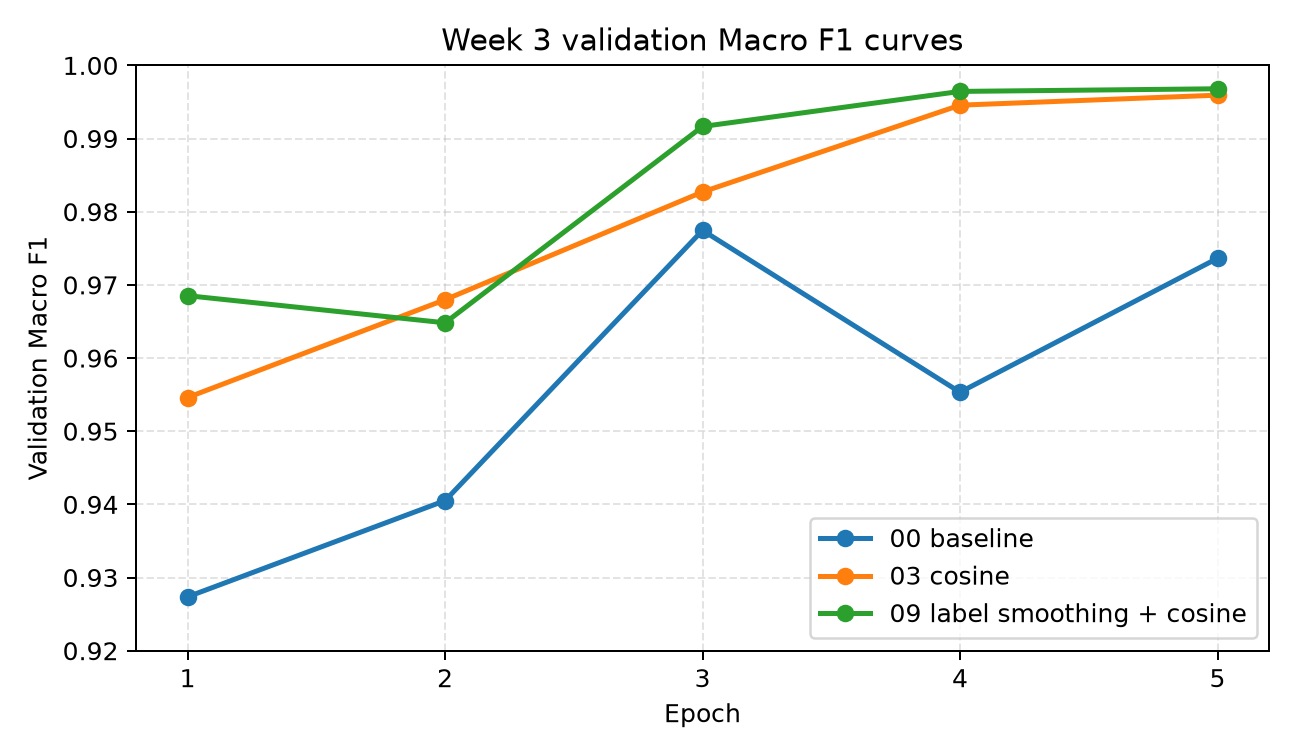
\includegraphics[width=0.88\textwidth]{../../reports/figures/week3_validation_macro_f1_curves.png}
\caption{Week 3 validation Macro F1 曲线。曲线来自固定预算运行；它展示优化过程，不消除单 seed 限制。}
\label{fig:week3-curves-zh}
\end{figure}
\FloatBarrier

\section{可解释性、错误分析与校准}

最终候选在 \PDATestCount 个 official test 样本中出现 \PDAErrorCount 个错误。主要混淆集中于视觉相似病害，例如玉米灰斑病与北方叶枯病、马铃薯晚疫病与番茄晚疫病。高分并未消除少量高置信错误；阈值 0.8 下仍记录两例。逐样本审计比单个 Accuracy 更能揭示系统何时可能自信地失败。

\begin{table}[htbp]
\centering
\caption{Week 4 错误与 top-label 校准审计（official split）}
\label{tab:week4-analysis-zh}
\begin{tabular}{p{0.44\textwidth}p{0.42\textwidth}}
\toprule
审计项 & 观测结果 \\
\midrule
测试错误 & 50 / 10709 \\
高置信错误（阈值 0.8） & Potato late blight $\rightarrow$ Tomato late blight（0.8475）；Apple scab $\rightarrow$ Apple healthy（0.8322） \\
Top-label calibration & ECE 0.0965；MCE 0.3348；Brier 0.0140 \\
解释边界 & 仅衡量预测标签置信度；不等同于完整多类别校准或田间可靠性 \\
\bottomrule
\end{tabular}
\end{table}


Top-label ECE 为 \PDAECE，MCE 为 \PDAMCE，Brier score 为 \PDABrier。多数样本位于高置信区，且该区 accuracy 高于平均 confidence，表现为 official split 上相对保守；低置信 bin 样本很少，因此不能过度解释 MCE 峰值。未执行 temperature scaling，也未评估完整的多类别校准。

\begin{figure}[tbp]
\centering
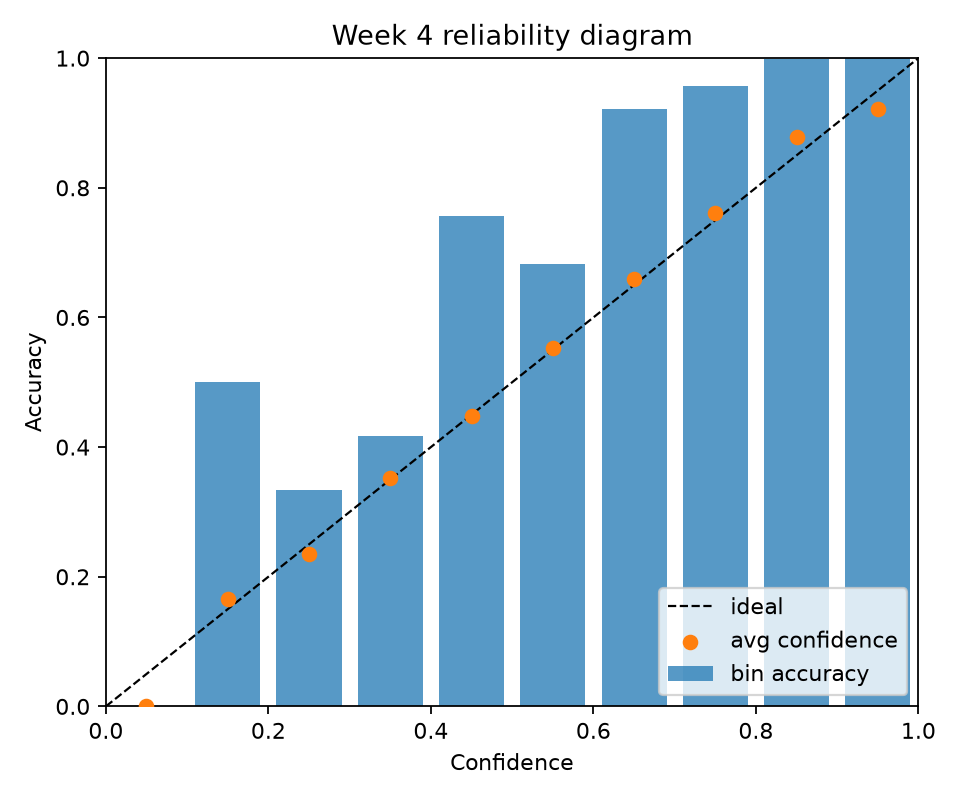
\includegraphics[width=0.63\textwidth]{../../reports/figures/week4_reliability_diagram.png}
\caption{Week 4 top-label reliability diagram。横轴为预测标签置信度，纵轴为正确率；图不表示田间可靠性。}
\label{fig:week4-reliability-zh}
\end{figure}

Grad-CAM 的正式目标层从 bottleneck 内部的 \texttt{layer4.2.conv3} 修正为 residual addition 之后的 \texttt{layer4.2}。修正改变了热力图观察，但不证明模型具有因果解释或没有背景偏差。24 样本 atlas 覆盖正确/错误和高/低置信四组；人工关注区域模板已经生成，但完整逐图审阅仍未完成。

\subsection*{三角证据而非漂亮案例}

固定 atlas 避免只挑选视觉上漂亮的热力图。正确高置信组检查激活是否位于叶片，错误高置信组暴露“自信但看错”的关注，低置信组呈现弱证据。每项记录 checkpoint、预处理、目标类别、目标层和样本索引。完整审阅应允许病斑、健康组织、边缘、背景、混合与不确定标签，并报告审阅者一致性。

校准与 Grad-CAM 回答不同问题。概率校准不说明哪些像素产生影响；叶片中心热力图也不保证输出正确或校准。错误数描述结果失败，却不描述空间机制。因此三类材料只能相互补充，不能互相替代；任何数值化解释评分都应在查看案例前预注册规则。

\begin{figure}[tbp]
\centering
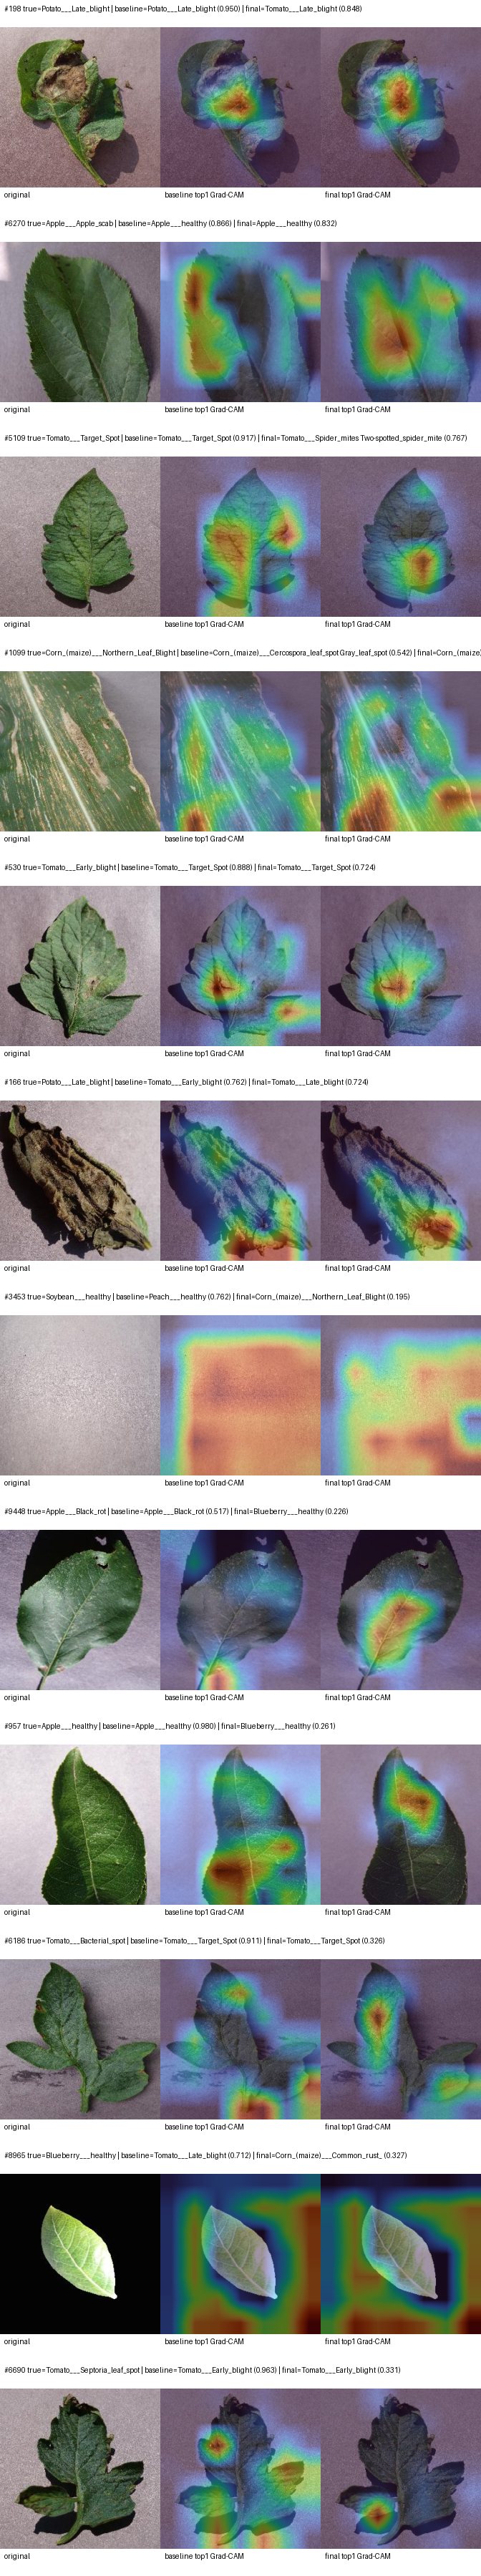
\includegraphics[height=0.62\textheight]{../../reports/figures/week4_baseline_vs_final_gradcam.png}
\caption{基线与最终候选的固定样本 Grad-CAM 对照。热力图表示相关性，不是病斑分割或因果证据。}
\label{fig:week4-gradcam-zh}
\end{figure}
\FloatBarrier

\section{Demo、MPS 服务与 Apple Container}

Week 5 把字节输入校验、Top-5 排序、概率与标签映射、低置信警告、Grad-CAM overlay 和非专业诊断声明封装到 UI 无关服务，再由 Streamlit 调用。Week 8 新增 React/Vite Liquid Glass 界面，仍复用同一冻结 checkpoint、标签与预处理。固定合成输入只验证历史工程路径；新界面的用户田间样例 SHA-256 为 \nolinkurl{0364ff44229c70666216343057f9ae77d82438a7f842b30af1ffabb786061a7e}，属于 out-of-domain 样例且 no verified ground truth。

\subsection*{分层服务与拒识}

React/FastAPI 路径现在先选择一片目标叶片，再运行模型。系统可自动接受明显占优的叶片组件，也可接收一个原图归一化坐标点；随后检查点击包含、前景保留、覆盖率、边缘接触和长叶主轴纯度。mask 失败或多叶歧义会返回明确的点选请求，而不是把整图强制送入分类器。通过门控后的中性背景 cutout 同时提供给植物身份、病害分类与 Grad-CAM，使手、土壤、天空和相邻植物不直接暴露给这些模型。

身份路由首先使用由 UCI Leaf100 与 14 个 PlantVillage 宿主组成的本地 114 类目录。它扩展的是路由词表，不是已验证的 114 物种开放世界准确率。仅当本地结果不确定且已配置密钥时，才调用可选 Pl@ntNet。PlantVillage 不支持的身份可以保留为身份观察，但病害路径必须拒答。对于支持宿主，OpenCV 在显示作物内 condition 概率前，独立记录异常覆盖率、主轴方向、形状、粗粒度颜色与空间分布。

接受为 Corn 的输入还要通过一个中轴形态门控。它在选择传染性 condition 之前检查异常覆盖率、中轴占比、纵向连续性、双侧相似度与离轴离散病斑。阳性形态会清除传染性标签、疾病知识、诊断 Grad-CAM 和管理建议资格，只显示 \texttt{suspected\_abiotic\_nutrient\_stress}。这是保守的安全提示，不是确诊缺氮。本地 Qwen 只描述可见形态；只要身份、condition 或非生物证据不支持病害声明，可选云端管理建议就保持锁定。

\begin{figure}[tbp]
\centering
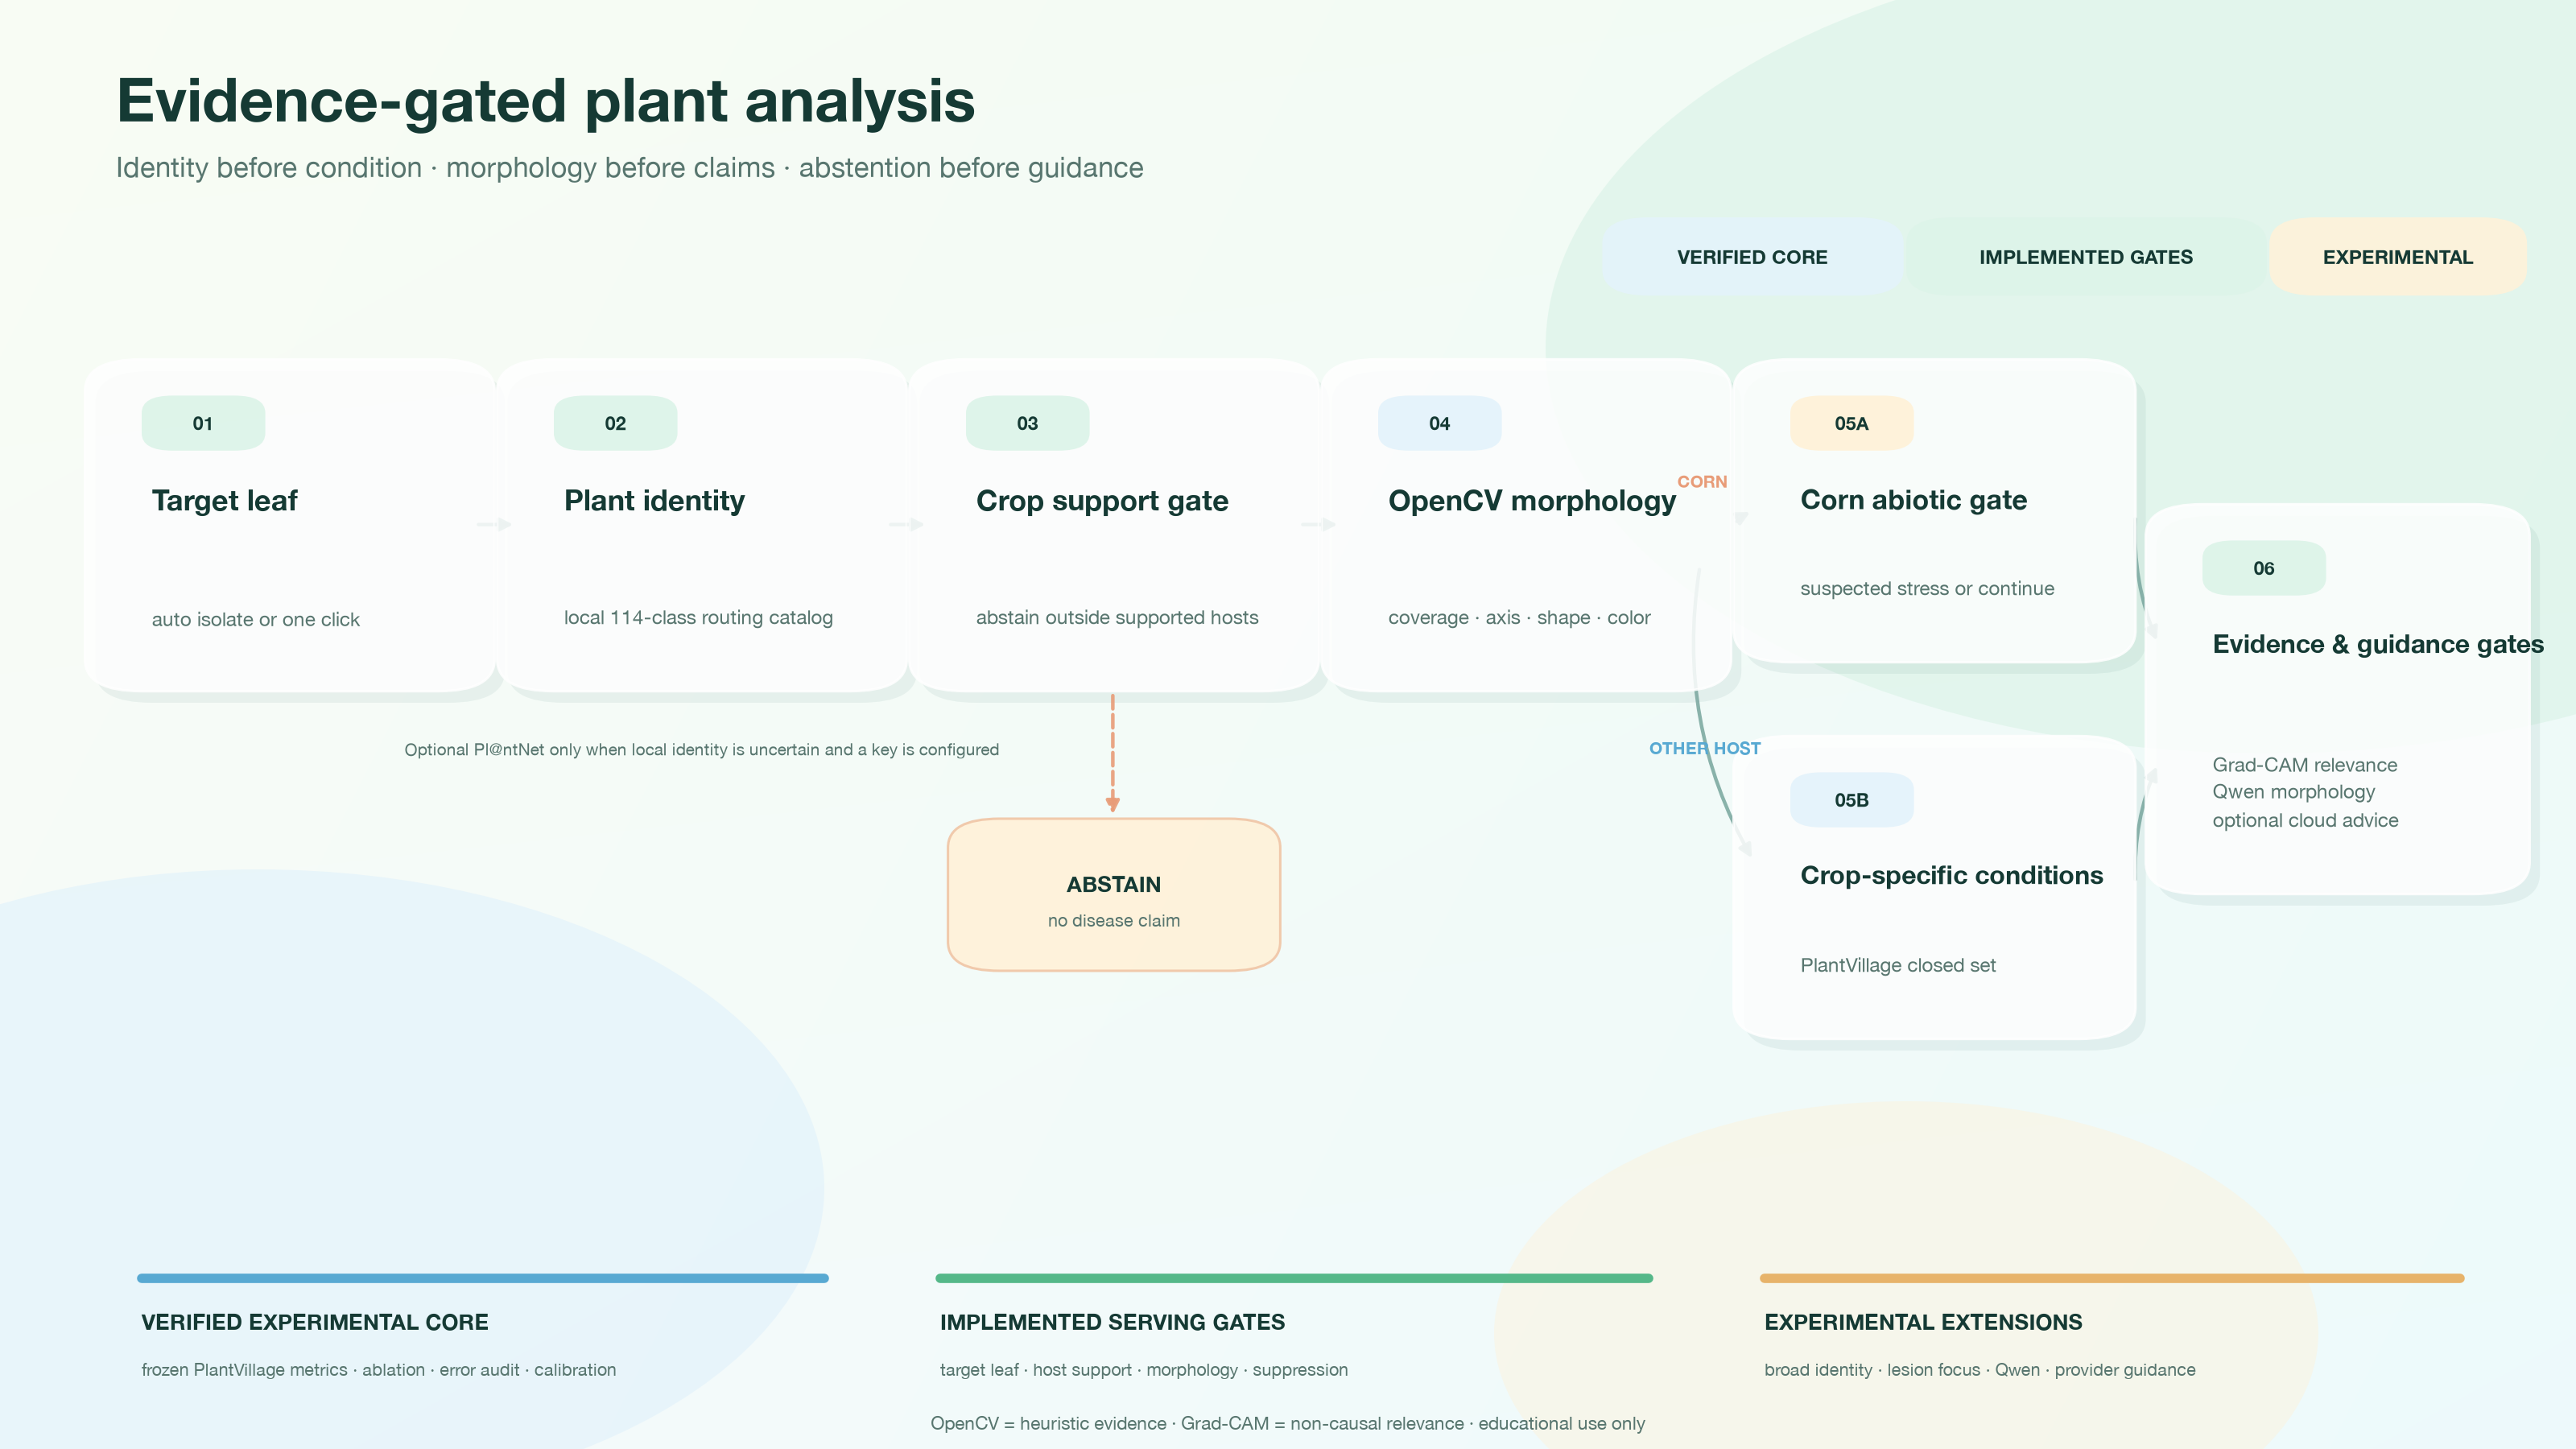
\includegraphics[width=0.98\textwidth]{../../docs/media/week8_hierarchical_serving_architecture.png}
\caption{冻结分类器外围已实现的分层服务与安全门控。该图不代表已验证开放世界身份准确率、病理分割或具体营养缺乏确诊。}
\label{fig:hierarchical-serving-zh}
\end{figure}

\begin{figure}[tbp]
\centering
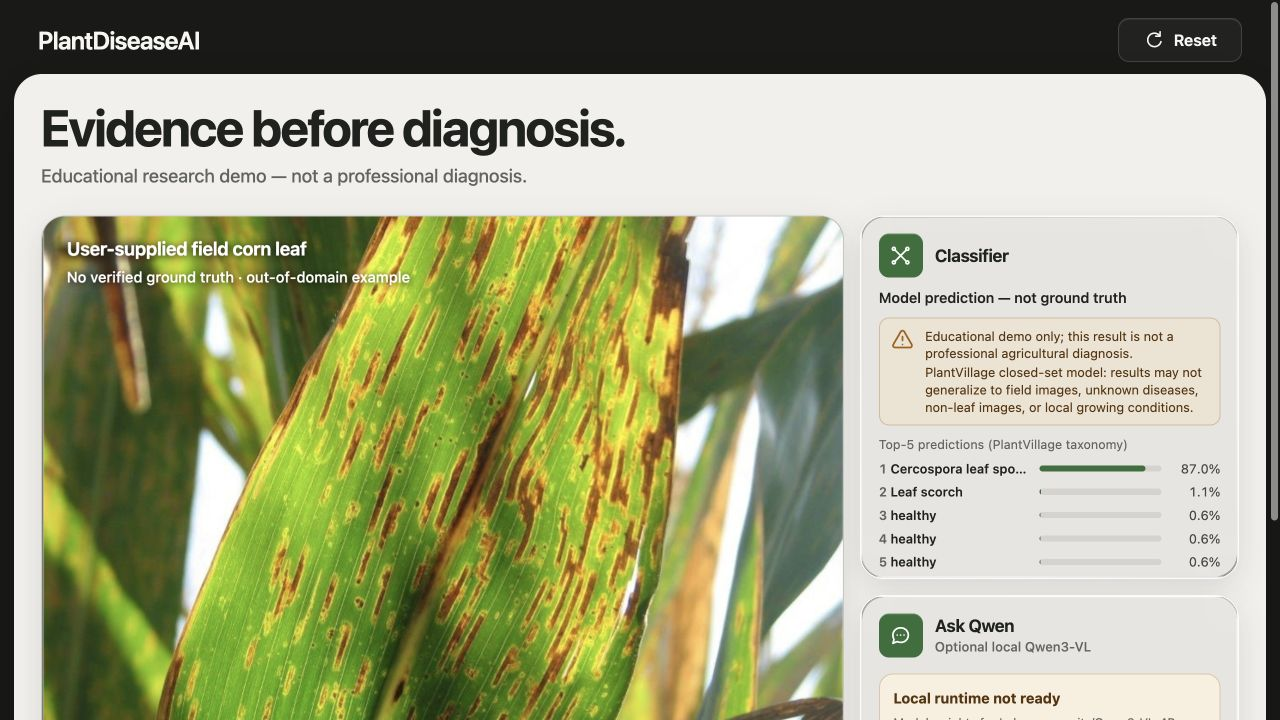
\includegraphics[width=0.94\textwidth]{../../reports/figures/week8_react_demo_desktop.png}
\caption{Week 8 React Demo 的浏览器审计截图。ResNet-50/MPS 输出的 0.870144 仅为 prediction，不是真值或田间准确率证据；图像无核验标签且超出 PlantVillage 受控背景域。}
\label{fig:week8-react-demo-zh}
\end{figure}

MPS 用于本机推理与 Week 8 本地证据重算。Apple container 运行 linux/arm64 CPU 镜像，模型权重通过只读式本地挂载进入容器。Week 5 记录的 \PDADemoLatency~ms 是容器内一个固定合成输入的单次总耗时，包含预测与 Grad-CAM；它不是重复冷启动、跨设备或生产负载 benchmark。Week 8 另一次 MPS fixed-demo 观测为 246.9~ms，两者条件不同，不应相互替代。

\subsection*{服务边界与运行失效}

服务在推理前拒绝空、损坏和过大的字节输入。低置信会追加警告，但置信度无法识别所有分布外输入；非叶片图片仍可能因 softmax 闭集而得到某个类别。因此界面独立于阈值声明 PlantVillage 域，并把 Top-5 视为模型输出而非鉴别诊断。

容器减少环境漂移，也引入边界：linux/arm64 CPU PyTorch 不能像 macOS 原生进程一样使用宿主 MPS。模型挂载、端口、架构、镜像 digest 与健康端点都是证据。生产研究还需并发、内存、启动分布、异常请求压力与可观测性测试；当前 health probe 不支持这些推论。

\section{Qwen3-VL 探索与安全边界}

Week 6 在分类主线完成后探索 Qwen3-VL-4B-Instruct 的本地 4-bit MLX 运行。VQA 数据按源图像实体分组，问题只覆盖植物、PlantVillage condition 与健康状态。Week 8 可选面板连接 \nolinkurl{mlx-community/Qwen3-VL-4B-Instruct-4bit}；浏览器审计时默认缓存权重缺失、\texttt{ready=false}，仅验证 UI unavailable state，浏览器/API no automatic download。对开放农业建议设定拒答：分类器低置信度不得被包装为确定诊断，涉及农药、剂量、法规和高风险处置时应咨询当地植保专家。

\begin{table}[htbp]
\centering
\caption{Week 6 Qwen3-VL 小样本冒烟比较（5 张图像、15 个问题）}
\label{tab:week6-vlm-zh}
\begin{tabular}{lrrp{0.35\textwidth}}
\toprule
提示方式 & 严格匹配 & condition & 证据边界 \\
\midrule
short free-form & 10/15 & 0/5 & 格式改善，但出现无依据病原术语 \\
choice & 11/15 & 1/5 & 自动风险词标记为 0；细粒度类别仍弱 \\
few-shot choice & 11/15 & 1/5 & 与 choice 持平；不是微调结果 \\
\bottomrule
\end{tabular}
\end{table}


choice 与 few-shot choice 均获得 \PDAVLMChoice 严格匹配，其中 plant 与 health status 各为 5/5，但细粒度 condition 仅 \PDAVLMCondition。short free-form 为 10/15，并出现病毒、真菌或细菌等未受支持术语。结构化选择减少了自由生成风险，却没有解决细粒度病害识别。由于只覆盖 5 张图像、15 个问题，且没有 LoRA/QLoRA 训练、完整人工评分或独立田间测试，本文只使用“smoke exploration”。

\subsection*{完整 VLM 评估需要什么}

严格匹配能发现闭集格式错误，却不适合开放解释。完整协议应冻结实体隔离图片，定义可接受同义词，并用盲审 rubric 评估正确性、图像 grounding、无依据病原结论、拒答质量及其与分类器置信度的一致性；自动指标旁还要报告审阅者一致性与失败案例。建议类问题必须先有可靠知识来源和辖区安全规则。

Few-shot prompting 只改变上下文，不是参数训练。LoRA/QLoRA 需要版本化训练集、实体隔离测试、adapter 配置、资源日志，以及对 zero-shot 和 classifier-assisted baseline 的固定比较。由于这些产物不存在，本文明确排除“完成微调”或“能力提升”的说法。

\section{Week 8 复现审计}

Week 8 release candidate 分为三条相互补充的本地通道。clean reproduction 从锁定依赖开始运行静态检查与完整测试；local evidence 使用冻结 checkpoint 重算指标、Top-5、MPS Demo 和 Grad-CAM atlas；Apple container 构建 linux/arm64 镜像并通过 Streamlit health probe。三条通道只证明当前本机与记录环境中的可复现状态，不等于公开部署可用性。

\begin{table}[htbp]
\centering
\small
\caption{Week 8 本地 release candidate 复现通道}
\label{tab:week8-repro-zh}
\begin{tabular}{lp{0.19\textwidth}p{0.49\textwidth}}
\toprule
通道 & 状态 & 实际证据 \\
\midrule
clean reproduction & passed & 锁定环境同步、226 项测试、Ruff 与 ty 静态检查通过 \\
local evidence & passed & 固定 checkpoint 重算指标、Top-5、MPS Demo 与 24 样本 Grad-CAM atlas \\
Apple container & passed & linux/arm64 镜像构建、Streamlit 健康检查与本地模型挂载通过 \\
\bottomrule
\end{tabular}
\end{table}


历史 clean lane 的 \PDAWeekEightCleanTests 项测试通过。当前交付 manifest 记录刷新后的源码、环境、锁文件、checkpoint 与跟踪产物。clean、package、local-evidence 和 container 在该源码上均为 \texttt{not\_run}，不继承历史通道证据；历史记录见 \texttt{reports/week8\_reproducibility.md}。claim ledger 将公开数字映射到证据文件并检查本地链接。该候选未创建或发布远程 release。

这种审计设计把“能跑”拆成可判定事件：环境是否能同步，代码检查是否通过，固定权重是否产生一致指标，解释与 Demo 是否生成，容器是否健康。它也保留未执行状态与限制字段，避免把未运行任务默认为成功。

\subsection*{来源追踪与 claim 控制}

release candidate 分开 Git 跟踪证据与大型本地产物。checkpoint 不进入普通源码历史，但由逻辑路径、大小和 SHA-256 标识；报告与展示输入采用相同方式。审阅者能发现模型或锁文件变化，同时不会泄露个人绝对路径。缺失必需产物会使候选失败，而不会用估计值补齐。

claim ledger 把锁定数字与允许措辞映射到证据并检查链接。限制语尤其需要该机制：0.9953 只能伴随 seed 42 与 official split；129.8~ms 必须保留固定合成 CPU 输入限定。机器检查无法判断所有修辞暗示，因此论文与 PPT 仍需人工证据审阅。

\section{讨论与负结果}

最重要的技术发现不是某个模型绝对最好，而是不同证据支持不同决策。ResNet50 支持高精度研究主线；MobileNetV2 支持资源权衡；Cosine Scheduler 在短预算下改善优化路径；Label Smoothing 改善监督目标。Focal Loss、EMA、RandAugment 与 Random Erasing 的下降同样限制了下一步搜索空间，说明“常用技巧”必须在冻结协议下验证。

错误、校准与 Grad-CAM 共同显示：Accuracy 不足以概括可靠性。50 个错误中存在高置信失败；ECE/MCE 依赖 bin 与 top-label 定义；解释目标层会显著改变热力图。把三者组合起来能提出更具体的后续问题，却仍不能给出因果结论。

VLM 结果也体现了负结果价值。封闭选项把严格匹配提高到 11/15，并移除自动风险词，但 condition 仍为 1/5。更流畅的自然语言并未转化为更可靠的病害识别。因此 VLM 适合作为带结构化上下文与拒答的交互分支，不能替代已经验证的分类器主线。

这些发现支持一个更普遍的方法论：可复现农业 AI 是循环，而不是从模型到 Demo 的单向流程。数据风险改变评估语言，错误模式提出新划分，解释层修正改变观察协议，服务失效又生成新测试。Week 8 在本地关闭当前循环，同时保留驱动下一循环的问题。

\section{局限、伦理与预期用途}

本研究有十一项核心限制。第一，official split 有 \PDAOfficialOverlap 个 leaf\_id 重叠；尚无实体隔离结果。第二，最终候选只有 seed 42，未报告多 seed 均值与方差。第三，PlantVillage 背景受控，未完成真实田间外部验证。第四，Grad-CAM 是相关性可视化，不是因果解释、分割或病理证据。第五，24 样本 attention review 和 72 项 VQA 模板尚未完成全量人工审计。第六，校准只覆盖 top-label，尚无 temperature scaling。第七，容器与本地延迟是特定条件观测，不是生产 SLA。第八，OpenCV 的目标叶片与病斑区域是启发式估计，不是专家标注的病理 mask。第九，114 类目录只有受控来源 pilot，没有已验证的 114 物种田间准确率。第十，Corn 门控没有专家标注的营养数据集，不能确认缺氮或其他具体原因。第十一，用户最初提供的缺氮图片已不在仓库中，因此现有门控 QA 不是对该精确文件完成的外部图像 Benchmark。

预期用途是研究、教学和工程展示：比较训练策略、演示闭集 Top-5、检查错误与解释产物、验证本地复现流程。非预期用途包括独立田间确诊、未知病害排除、农药选择与剂量、法规建议、商业生产决策或人身/生态高风险处置。界面和材料必须保留“非专业诊断”声明，并在低置信、超范围或高风险问题上拒答。

数据、模型与第三方依赖应按各自许可使用。论文只引用公开的一手论文或模型卡；本地权重、原始数据和用户路径不进入 Git。自动化写作不能改变实验事实，所有最终论断必须回到机器可读结果、日志、图表或审计报告。

下一研究应在训练前预注册实体键与 split，保留完全未触碰的最终测试域，并在相同预算下运行多个固定 seed。报告应包含 Accuracy/Macro F1 均值与离散程度、分类别不确定性和全部失败运行。田间子集要覆盖光照、杂乱背景、视角、作物阶段和采集设备，并记录授权与许可。这些步骤能把当前限制变成可检验研究假设，而不是只存在于展示材料中的免责声明。

\section{结论与未来工作}

PlantDiseaseAI 已形成从数据审计、统一基准、消融选择、逐样本错误、校准、Grad-CAM，到 MPS Demo、Apple container、VLM 冒烟、Week 8 release audit 与后续证据门控 React/FastAPI 服务架构的本地闭环。当前候选在 seed 42 official split 上达到 \PDAFinalAccuracy{} Accuracy 与 \PDAFinalMacroFOne{} Macro F1；这一数字与 \PDAOfficialOverlap{} 个实体重叠风险必须同时呈现。项目的研究价值来自证据边界，而不是把高分、启发式 mask 或广域身份目录扩写成田间可信性。

下一阶段优先级依次为：建立 leaf entity 隔离的冻结 split；运行多个随机种子并报告离散程度；收集有合法来源的田间域样本；建立专家标注的生物、非生物与营养胁迫区域数据；以区域标注评估目标叶片与病斑 mask；完成 Grad-CAM/VQA 人工审计；评估拒答与开放集输入；只在资源与固定测试协议允许时研究 LoRA/QLoRA。任何新结果都应进入版本化 manifest 与 claim ledger，再进入论文、PPT 或简历。

\section*{工具披露}

Codex 被用于代码与文档辅助、结构检查和构建自动化。作者 Panjoel 对实验设计、证据选择、结果解释、文字定稿与全部研究责任负责；Codex 不是共同作者。

\bibliographystyle{plain}
\bibliography{../references}

\end{document}
